% Anonymised review copy for JASSS referees.
% Compile with pdfLaTeX + BibTeX from this directory (or Overleaf).

\documentclass{JASSS}

\title{The Polarization Paradox: How Suppressing Backfire Cascades Entrenches Ideological Segregation under Fragile Trust}

\reviewcopy{true}

% Authors retained in source for the author PDF; suppressed by \reviewcopy{true}
\author[1]{Anonymised}
\affil[1]{Anonymised}
\email{anonymised@example.com}

\usepackage{natbib}
\setcitestyle{authoryear,round,aysep={}}

\usepackage{amssymb}
\usepackage{booktabs}
\usepackage{hyperref}
\usepackage{url}
\usepackage{microtype}
\usepackage[font=small,labelfont=bf]{caption}

\graphicspath{{../}{./}}

% Flag consumed by section files to strip identifying URLs
\newcommand{\BlindSubmission}{}

\begin{document}
\maketitle

\begin{abstract}{%
In modern social media platforms, toxic polarization drives user frustration and permanent churn, threatening brand safety and platform advertising revenue. To combat this, digital platforms increasingly deploy content moderation interventions such as bridging algorithms, which suppress confrontational, cross-cutting interactions that fall into users' ``latitude of rejection.'' Using the Dynamic-BABE (Biased Assimilation \& Behavioral Entrenchment) agent-based model, we examine the systemic consequences of such algorithmic interventions in the context of co-evolving dyadic trust. We discover a critical counter-intuitive phenomenon: the Polarization Paradox. While the bridging algorithm successfully curtails behavioral frustration and drops cumulative user churn from 39.18\% to 0.38\% (Cohen's $d = 23.97$, $p < 0.001$), preserving platform revenue (increasing from \$121.64 to \$199.24), it simultaneously exacerbates systemic ideological division. Specifically, we find that polarization increases from 0.9550 to 0.9904 (Cohen's $d = -1.28$, $p < 0.001$). By suppressively shielding agents from disagreeable outgroup opinions, the algorithm prevents the constructive exposure necessary to cultivate tolerance and build dyadic interpersonal trust. Under fragile trust, the absence of direct engagement induces trust segregation---wherein trust concentrates exclusively within homogeneous echo chambers while outgroup relationships wither. Consequently, the network undergoes social fragmentation and structural entrenchment. Our results demonstrate that platforms face a fundamental trade-off: short-term economic stabilization and customer retention are achieved at the cost of long-term democratic cohesion, suggesting that superficial moderation fails to resolve the deep-seated cognitive and relational dynamics of online polarization.
%
}
\end{abstract}

\begin{keywords}{agent-based modeling; opinion dynamics; polarization; dyadic trust; algorithmic curation; social media}
\end{keywords}

\parano{}

\section{Introduction}
\label{sec:intro}
The rapid ascendancy of social media platforms has radically restructured the architecture of modern human communication, shifting public discourse from local physical spaces to global digital environments. While these platforms were initially championed as instruments of democratic liberation and social connection, they are increasingly scrutinized for their role in fostering severe ideological and affective polarization \cite{Bail2018, Levy2021}. In these virtual arenas, disagreement is frequently amplified, leading to a fragmented public square characterized by echo chambers, mutual distrust, and hostile interactions. 

For social media firms, systemic polarization is not merely a regrettable social externality; it represents a profound threat to their core economic models. When digital environments become excessively hostile, users experience cumulative cognitive fatigue and emotional distress, leading to permanent exit from the platform---a phenomenon described in classic economic theory by \cite{Hirschman1970} as the ``exit'' option. Under severe polarization, user churn accelerates, directly reducing the active user base and eroding the platform's primary source of monetization: ad impressions. Furthermore, heightened toxicity and extreme discourse trigger a ``brand safety penalty'' \cite{Guess2023}. Advertisers, highly sensitive to reputational risks, increasingly restrict or withdraw their ad spend from platforms that fail to maintain a civil and safe environment. Consequently, social media corporations face a critical imperative to deploy algorithmic moderation strategies to maintain user retention and stabilize advertising revenue.

To combat this toxic churn, platforms have turned to algorithmic interventions. Historically, moderation focused on reactive ex-post content removal or account suspensions. More recently, however, platforms have begun experimenting with structural feed interventions, such as ``bridging algorithms'' \cite{Guess2023}. These recommendation systems seek to identify and suppress confrontational, cross-cutting content that is highly likely to trigger negative cognitive responses and aggressive exchanges. From a psychological standpoint, such interventions target the ``latitude of rejection'' \cite{Sherif1961}---the zone of opinions so divergent from an individual's prior beliefs that exposure causes cognitive backlash and opinion repulsion (the backfire effect) rather than assimilation. By suppressively filtering these hostile, backfire-inducing interactions, bridging algorithms seek to lower user frustration, minimize churn, and maintain a brand-safe digital ecosystem.

Yet, this study uncovers a profound and counter-intuitive tension between platform economics and systemic social dynamics, which we define as the \textit{Polarization Paradox}. While bridging algorithms are highly effective at achieving their immediate goals---successfully curbing user frustration, reducing churn, and preserving platform revenue---they simultaneously entrench and exacerbate systemic polarization. We argue that by shielding individuals from disagreeable, cross-cutting interactions, bridging algorithms prevent the constructive tension necessary for the cultivation of interpersonal tolerance and mutual trust.

We formalize this thesis by introducing a novel agent-based simulation framework: the Dynamic-BABE (Biased Assimilation \& Behavioral Entrenchment) model. Our framework extends classical models of opinion dynamics, such as the DeGroot consensus model \cite{DeGroot1974} and the Hegselmann-Krause bounded confidence model \cite{Hegselmann2002}, by integrating the entrenchment-based biased assimilation formulation of Chen et al. \cite{Chen2021} with Social Judgment Theory \cite{Sherif1961, Jager2005} and a co-evolving network of dyadic interpersonal trust. Crucially, trust in our model is not a static network parameter but a dynamic, dyadic property that co-evolves with opinion interactions. Consistent with empirical findings from risk and trust research \cite{Slovic1993}, trust is fragile: it builds slowly upon successful consensus-seeking interactions but erodes rapidly when confrontational, backfire-inducing exchanges occur.

Through a rigorous 2$\times$2 factorial experiment crossing the activation of the bridging algorithm and dynamic trust, we demonstrate that when dyadic trust is fragile, the suppression of confrontational cross-cutting interactions deprives agents of the opportunity to build mutual tolerance. When the bridging algorithm is active, agents are effectively insulated from their ideological opponents. While this dampens immediate conflict and eliminates the frustration that triggers churn, it also prevents the successful, low-friction interactions that allow trust to rebuild across ideological lines. Over time, relations that are not actively maintained wither due to passive relational decay. The network consequently undergoes \textit{trust segregation}---a state where trust is highly concentrated within homogeneous opinion clusters, while trust between opposing groups completely collapses. Ultimately, this trust segregation locks the society into a structurally entrenched state of polarization.

The contributions of this paper are threefold. First, we develop the Dynamic-BABE model, a novel ABM that bridges cognitive psychology, relational network dynamics, and platform economics. Second, we empirically demonstrate the existence of the Polarization Paradox, illustrating the severe trade-off platforms face between short-term financial sustainability and long-term social cohesion. Finally, we highlight the dangers of purely suppressive, content-centric algorithmic moderation, arguing that meaningful solutions to online polarization must move beyond simple avoidance mechanisms toward interventions that foster relational trust and mutual tolerance.


\section{Related Work}
\label{sec:related}
We situate Dynamic-BABE in five literatures: classical opinion dynamics, biased assimilation, Social Judgment Theory, co-evolving trust, and algorithmic exposure.

\subsection{Classical Models of Opinion Dynamics}
\citet{DeGroot1974} modelled influence as repeated weighted averaging. In a connected network this process converges to consensus, which cannot explain persistent disagreement. Bounded-confidence models restrict influence to neighbours within a similarity threshold~\citep{Hegselmann2002, Deffuant2000} and can produce multiple clusters. \citet{Flache2017} review these and related formalisms. Bounded confidence typically ignores out-of-range neighbours rather than modelling active repulsion, and classical OD usually lacks an exit channel that changes the communicating population.

\subsection{Cognitive Resistance and Biased Assimilation}
\citet{Lord1979} showed that people can interpret mixed evidence in ways that strengthen prior attitudes---biased assimilation. \citet{Dandekar2013} embedded related biases in network models and linked them to polarization under homophily. \citet{Chen2021} proposed BEBA, where influence weights $w_{ij}(t) = 1 + \beta_i y_i(t) y_j(t)$ depend on entrenchment $\beta_i$ and alignment, so negative influence can emerge endogenously. \citet{Mas2013} discuss bipolarization without explicit distancing. We adapt Chen-style weights to pairwise, multi-issue interactions, map them onto Social Judgment zones~\citep{Sherif1961, Jager2005}, and add co-evolving dyadic trust.

\subsection{Social Judgment Theory and Backfire}
Social Judgment Theory partitions attitude space into latitudes of acceptance, non-commitment, and rejection~\citep{Sherif1961}. Messages in the acceptance latitude tend to pull opinions toward the source; messages in the rejection latitude can produce contrast and backlash. Empirical evidence for attitude \emph{backfire} / boomerang effects is contested: some exposure regimes raise extremity~\citep{Bail2018}, while feed and correction experiments often find null or highly context-dependent attitude change~\citep{Guess2023, Levy2021}. We treat Zone~3 repulsion as a modelled Social Judgment mechanism, not as an empirical universal. \citet{Jager2005} showed that repulsion in networks can create opposing camps. We treat influence weights as determining these zones.

\subsection{Networks and Dyadic Trust}
Opinions and social structure often co-evolve~\citep{Macy2002, Centola2010, Keijzer2018}. Many models allow rewiring toward similar others. We hold the undirected graph fixed and instead let edge trust change with interaction. Trust is asymmetric in gain and loss~\citep{Slovic1993}: it rises slowly after agreement and falls faster after conflict. High trust buffers occasional disagreement; low trust makes further conflict more likely.

\subsection{Algorithmic Interventions, Filtering, and Exposure}
Platforms once hoped that cross-cutting exposure would reduce polarization. \citet{Bail2018} found that exposing Twitter users to opposing-party bots could increase extremity. Feed experiments also show that ranking regimes change on-platform behavior, often more than deep attitudes~\citep{Levy2021, Guess2023}. On the modelling side, algorithmic bias in partner selection can amplify fragmentation and polarization in bounded-confidence settings without modelling exit~\citep{Sirbu2019}; adaptive-network work often rewires ties~\citep{Macy2002, Keijzer2018}. What those neighbours do not jointly deliver---and what we treat as the paper's single distinctive claim---is a suppression filter coupled to Hirschmanian exit so that \emph{retention rises while active-set $\sigma$ stays high or rises}, with $\sigma_{\mathrm{all}}$ showing that the rise is survivorship rather than population warming, plus a \emph{separate} trust-segregation axis on fixed topology. We abstract suppression as a probabilistic filter that intercepts rejection-zone events---distinct from ranking that \emph{promotes} like-minded contact~\citep{Sirbu2019} or constructive bridging. We use ``Polarization Paradox'' for that retention-versus-survivor-dispersion tension without claiming uniqueness of the name. Field studies rarely observe long-run feedback among opinions, trust, and exit; the ABM is built for that gap.


\section{Model Description (ODD+D Protocol)}
\label{sec:model}
% paper/sections/04_method_odd.tex
% Method Section following the ODD+D Protocol

The model presented in this study, the Dynamic-BABE (Biased Assimilation \& Behavioral Entrenchment) model, is reported here following the standardized ODD+D (Overview, Design concepts, Details, and Decision-making) protocol \citep{Grimm2010, Muller2013}. This protocol provides a structured framework to describe agent-based models, focusing on human decision-making and cognitive processes, which are central to social media opinion dynamics.

\subsection{Overview}

\subsubsection{Purpose}
The primary purpose of the Dynamic-BABE model is to investigate the complex, co-evolutionary feedback loop between interpersonal dyadic trust, individual cognitive processes of opinion dynamics (biased assimilation and backfire effects), and platform-level algorithmic moderation (specifically, bridging algorithms). By simulating these interconnected dynamics, the model aims to explain the ``Polarization Paradox''---a systemic phenomenon where platform moderation strategies succeed in keeping users active and retaining ad revenue in the short term, but paradoxically exacerbate long-term ideological segregation and trust polarization.

\subsubsection{Entities, State Variables, and Scales}
The model consists of two primary classes of entities: \textbf{agents} (representing individual social media platform users) and the \textbf{network environment} (representing the social network structure and the platform's computational layer).

\paragraph{Agents:} Each agent $i \in \{1, 2, \dots, N_{\text{agents}}\}$ represents a platform user and is characterized by the following state variables:
\begin{itemize}
    \item \textbf{Opinion Vector} ($\vec{O}_i \in [-1, 1]^K$): A multi-dimensional real-valued vector representing the agent's ideological stance on $K$ distinct social or political issues. Each issue dimension $d \in \{1, \dots, K\}$ is scaled continuously from $-1.0$ (strongly progressive/left) to $+1.0$ (strongly conservative/right).
    \item \textbf{Salience Vector} ($\vec{S}_i \in [0, 1]^K$): A probability distribution vector representing the relative cognitive importance or attention weight that agent $i$ allocates to each of the $K$ issues. To ensure valid weighting across issues, the salience vector is constrained such that $\sum_{d=1}^K S_{i,d} = 1.0$.
    \item \textbf{Cognitive Entrenchment} ($\beta_i \in [\beta_{\min}, \infty)$): A positive scalar representing the agent's cognitive resistance, closed-mindedness, or susceptibility to confirmation bias \citep{Chen2021}. A higher value of $\beta_i$ indicates that the agent is more resistant to opinions discrepant from their own and more likely to experience backfire repulsion.
    \item \textbf{Behavioral Frustration} ($F_i \in \mathbb{N}_0$): A non-negative integer counter that accumulates cognitive dissonance and psychological irritation resulting from negative, confrontational cross-cutting interactions.
    \item \textbf{Active Status} ($\text{Active}_i \in \{\text{True}, \text{False}\}$): A boolean flag denoting whether the agent is currently participating in the social network. Agents permanently transition to $\text{Active}_i = \text{False}$ (user churn) when their frustration exceeds a critical threshold $T_c$.
\end{itemize}

\paragraph{Network and Platform Environment:} The social structure is represented as an undirected scale-free graph $G = (V, E)$ initialized using the Barab\'{a}si-Albert (BA) preferential attachment model \citep{Barabasi1999}, where $V$ represents the set of agents and $E$ represents the set of communication channels (edges). 
\begin{itemize}
    \item \textbf{Dyadic Interpersonal Trust} ($T_{ij} \in [0, 1]$): A real-valued symmetric weight assigned to each active edge $(i, j) \in E$. Trust represents the relational capital between agents $i$ and $j$, acting as a cognitive buffer that mitigates disagreement and co-evolves with opinion alignment. If trust is disabled, $T_{ij} = T_0 = 0.5$ for all edges.
    \item \textbf{Algorithmic Interception Layer}: The platform's algorithm which monitors dyadic interactions. If enabled, it probabilistically intercepts interactions destined to cause a backfire, neutralizing the negative impact.
\end{itemize}

\paragraph{Scales:} The temporal scale of the model consists of discrete simulation steps (ticks) $t \in \{1, 2, \dots, t_{\max}\}$. A single step represents an arbitrary communicative epoch (e.g., a day of activity on a social platform) during which agents select neighbors for dialogue. The spatial scale is topological, defined by the scale-free network topology. The population scale is parameterized at $N_{\text{agents}} = 500$ agents connected by a scale-free network with preferential attachment edge parameter $m_e = 3$.

\subsubsection{Process Overview and Scheduling}
In each discrete simulation step $t$, the schedule executes the following sequence of operations:
\begin{enumerate}
    \item \textbf{Randomized Activation Order:} The simulation scheduler constructs a randomized list of all active agents to prevent artifactual sequencing effects.
    \item \textbf{Agent Interaction Loop:} For each active agent $i$ in the randomized list:
    \begin{enumerate}
        \item The agent identifies the subset of its topological neighbors in $G$ who are currently active: $\mathcal{N}_i^{\text{active}}(t) = \{j \in \mathcal{N}_i : \text{Active}_j(t) = \text{True}\}$. If $\mathcal{N}_i^{\text{active}}(t)$ is empty, the agent skips its turn.
        \item The agent selects a subset of partners $\mathcal{P} \subseteq \mathcal{N}_i^{\text{active}}(t)$ of size $k = \min(k_{\text{step}}, |\mathcal{N}_i^{\text{active}}(t)|)$ uniformly at random without replacement. Under default parameters, $k_{\text{step}} = 1$.
        \item For each selected partner $j \in \mathcal{P}$, the directed interaction pipeline $\text{Interact}(i, j)$ is executed, wherein agent $i$'s opinion vector, frustration level, and active status are updated. In parallel, the symmetric dyadic trust $T_{ij}$ is co-evolved on the network edge.
    \end{enumerate}
    \item \textbf{Passive Trust Decay:} After all agents have executed their active interactions, the platform's relationship network experiences passive trust erosion due to neglect. For every edge $(u, v) \in E$, the dyadic trust decays by a fraction $\lambda$:
    \begin{equation}
        T_{uv}(t+1) = T_{uv}(t) \cdot (1 - \lambda)
    \end{equation}
    \item \textbf{Platform Diagnostics and Data Collection:} System-wide metrics (global polarization $\sigma(t)$, cumulative churn rate, average active user frustration, total active users, mean network-wide trust, ingroup/outgroup trust, trust segregation ratio, and opinion-weighted clustering) are computed and logged.
    \item \textbf{Termination Check:} If all agents have churned ($N_{\text{active}} = 0$) or the maximum step limit $t_{\max} = 200$ is reached, the simulation terminates.
\end{enumerate}

\subsection{Design Concepts}

\subsubsection{Theoretical Background}
The cognitive architecture of the Dynamic-BABE model is grounded in \textbf{Social Judgment Theory} \citep{Sherif1961, Jager2005}, which partitions an agent's attitude spectrum into three regions: the Latitude of Acceptance (assimilative change), the Latitude of Non-Commitment (no change), and the Latitude of Rejection (contrast effect / backfire). 

The mathematical formulation of cognitive entrenchment ($\beta_i$) and opinion alignment ($A_{ij}$) builds directly on the \textbf{Biased Assimilation and Behavioral Entrenchment (BEBA)} model proposed by \citet{Chen2021}, which extends the classical consensus model of \citet{DeGroot1974}. 

The co-evolution of dyadic trust is conceptually derived from social psychology and risk research by \citet{Slovic1993}, which posits that trust is asymmetrical: it is difficult to build but exceptionally easy to destroy. 

Finally, the relationship between user active status, frustration, and platform exit is mapped using the classic \textbf{Exit-Voice-Loyalty (EVL)} framework of \citet{Hirschman1970}.

\subsubsection{Individual Decision-Making}
The decision-making process of agents is represented by heuristic-driven cognitive updates rather than utility maximization. When agent $i$ is exposed to the opinion of agent $j$, it does not optimize a strategic payoff; instead, it updates its opinion $\vec{O}_i$ and frustration level $F_i$ automatically based on the cognitive alignment $A_{ij}$ and the resulting influence weight $w_{ij}$. 

The fundamental rule is:
\begin{itemize}
    \item If the perceived influence weight is high and positive ($w_{ij} > \tau_{\text{assim}}$), the agent enters its Latitude of Acceptance, experiences cognitive relief, and assimilates toward the sender.
    \item If the influence weight is moderate ($0 \leq w_{ij} \leq \tau_{\text{assim}}$), the interaction falls in the Latitude of Non-Commitment and is ignored.
    \item If the influence weight is negative ($w_{ij} < 0$), the interaction falls in the Latitude of Rejection, triggering a defensive backfire repulsion that pushes opinions further apart and increases behavioral frustration.
\end{itemize}

\subsubsection{Learning}
Agents do not engage in deep machine learning or reinforcement learning. However, they possess a relational memory represented by the dyadic trust weight $T_{ij}$ on the network edges. Agents ``learn'' about the reliability and ideological compatibility of their neighbors over time. Positive, assimilative interactions build trust slowly ($\delta_+$), while negative, backfiring interactions destroy trust rapidly ($\delta_-$). This co-evolutionary learning shapes the future influence of neighbors, creating a feedback loop between social network structure and opinion dynamics.

\subsubsection{Individual Sensing}
An agent $i$ has perfect local sensing of its direct topological neighbors in $G$. Specifically, when interacting with neighbor $j$, agent $i$ can sense $j$'s current opinion vector $\vec{O}_j$ and $j$'s salience vector $\vec{S}_j$. Agents cannot sense the opinions, saliences, or cognitive variables of non-neighboring agents, nor do they possess any global knowledge of the platform's aggregate polarization or network structure.

\subsubsection{Individual Prediction}
Agents are entirely reactive and operate without predictive capabilities. They do not forecast the future opinions of their neighbors, nor do they anticipate the risk of their own frustration exceeding the churn threshold.

\subsubsection{Interaction}
Interactions in the model are local, dyadic, and directional. While trust updates are symmetric across the edge $(i, j)$, the cognitive updates are executed from the perspective of the active agent $i$ receiving input from the passive partner $j$. 

Platform-level algorithmic moderation (the bridging algorithm) acts as a critical filter on these interactions. By suppressing backfire interactions, the platform actively intercepts and modifies the interaction outcomes, transforming a hostile backfire into a neutral event, thereby shielding users from frustration at the cost of genuine ideological resolution.

\subsubsection{Collectives}
No formal collectives (such as coalitions, parties, or organized groups) are explicitly represented in the model. However, functional collectives emerge endogenously as a result of opinion dynamics. Specifically, agents cluster into distinct ideological camps, which we identify as ``ingroup'' and ``outgroup'' structures based on the sign of their average opinion. These emergent collectives dictate the flow of trust and the formation of echo chambers.

\subsubsection{Heterogeneity}
Agents are highly heterogeneous across multiple dimensions:
\begin{itemize}
    \item \textbf{Ideological Stances:} Initialized bipolarly, splitting the population into two opposed camps with positive and negative opinions.
    \item \textbf{Issue Salience:} Agents care about different issues to different degrees, with saliences drawn from a Dirichlet distribution.
    \item \textbf{Cognitive Entrenchment:} Each agent has a unique $\beta_i$ drawn from a normal distribution, representing their varying degrees of dogmatism.
    \item \textbf{Network Topology:} Due to the scale-free Barab\'{a}si-Albert structure, agent degree is highly heterogeneous, with a few hub agents possessing exceptionally high connectivity and influence, while most agents have few connections.
\end{itemize}

\subsubsection{Stochasticity}
Stochasticity is deeply integrated into the simulation to model social noise and unpredictability:
\begin{itemize}
    \item The network topology is generated stochastically via BA preferential attachment.
    \item Agent activation order is randomized at the beginning of each time step.
    \item Dialogue partner selection is stochastic, with agents choosing randomly among active neighbors.
    \item The bridging algorithm is probabilistic, succeeding in intercepting a backfire with an efficacy rate of $E = 46\%$.
    \item Initialization of issue saliences ($\vec{S}_i$), entrenchment ($\beta_i$), and starting opinion vectors ($\vec{O}_i$) are governed by random draws from Dirichlet, Normal, and Uniform distributions, respectively.
\end{itemize}

\subsubsection{Observation}
System-level and agent-level data are collected at the end of each step. The primary observation variables are:
\begin{itemize}
    \item \textbf{Global Polarization ($\sigma(t)$):} Root-mean-square of issue-dimensional standard deviations.
    \item \textbf{Active User Count ($N_{\text{active}}$):} Total number of agents with $\text{Active}_i = \text{True}$.
    \item \textbf{Churn Rate:} Fraction of the population that has permanently exited.
    \item \textbf{Average Frustration:} Mean frustration level across active agents.
    \item \textbf{Platform Revenue ($R(t)$):} Aggregate step-wise ad revenue subject to brand safety penalties.
    \item \textbf{Trust Segregation Ratio:} Ratio of mean ingroup trust to outgroup trust.
    \item \textbf{Opinion-Weighted Clustering Coefficient:} Fraction of topological triangles sharing the same opinion pole.
\end{itemize}

\subsection{Details and Decision-Making}

This section details the governing mathematical equations and rules that define the initialization, dyadic interactions, trust co-evolution, user churn, and platform revenue.

\subsubsection{Initialization}
At time $t = 0$, a population of $N_{\text{agents}} = 500$ agents is placed on a Barab\'{a}si-Albert scale-free graph generated with preferential attachment parameter $m_e = 3$. 

The opinion vectors $\vec{O}_i \in [-1, 1]^K$ (for $K = 2$ issues) are initialized using a \textbf{bipolar split} to model a pre-polarized society:
\begin{equation}
    O_{i,d}(0) = \text{clip}\Big( \text{sgn}(\xi_i) \cdot U_i(0.4, 1.0) + \epsilon_{i,d},\, -1.0,\, 1.0 \Big)
\end{equation}
where $\xi_i \sim \mathcal{U}(-1, 1)$ is a uniform random scalar drawn for agent $i$ determining their ideological camp ($\text{sgn}(\xi_i) \in \{-1, +1\}$), $U_i(0.4, 1.0)$ is a uniform random draw representing their base camp intensity, and $\epsilon_{i,d} \sim \mathcal{N}(0, 0.05^2)$ is minor issue-specific individual noise. This splits the population roughly 50/50 into a left-pole camp and a right-pole camp.

Each agent's salience vector $\vec{S}_i$ is drawn from a symmetric Dirichlet distribution:
\begin{equation}
    \vec{S}_i \sim \text{Dirichlet}(\vec{\alpha})
\end{equation}
where $\vec{\alpha} = [1, 1]^T$ for $K = 2$ issues, ensuring that $S_{i,d} \in [0, 1]$ and $\sum_{d=1}^K S_{i,d} = 1.0$.

Cognitive entrenchment $\beta_i$ is drawn from a normal distribution and floored to prevent negative values:
\begin{equation}
    \beta_i = \max\Big( \beta_{\min},\, \nu_i \Big), \quad \nu_i \sim \mathcal{N}(\mu_{\beta},\, \sigma_{\beta}^2)
\end{equation}
with default values $\beta_{\min} = 0.5$, $\mu_{\beta} = 4.0$, and $\sigma_{\beta} = 1.5$.

Symmetric dyadic trust on all network edges $(u, v) \in E$ is initialized to a uniform starting value:
\begin{equation}
    T_{uv}(0) = T_0 = 0.5
\end{equation}
Behavioral frustration is initialized to $F_i(0) = 0$ for all agents.

\subsubsection{Dialogue Dynamics and Opinion Updates}
When agent $i$ is activated, it selects a random active neighbor $j$ and receives their opinion. The interaction is processed through a multi-stage cognitive pipeline.

\paragraph{Step 1: Salience-Weighted Opinion Alignment ($A_{ij}$)}
The cognitive distance between the active agent $i$ and the sender $j$ is calculated as a salience-weighted dot product. The alignment is given by:
\begin{equation}
    A_{ij} = \sum_{d=1}^K O_{i,d} \cdot \left(\frac{S_{i,d} + S_{j,d}}{2}\right) \cdot O_{j,d}
\end{equation}
This alignment formulation captures the psychological reality that issues of mutual importance (high salience) contribute disproportionately to the perceived agreement or disagreement. Because opinions are bounded in $[-1, 1]$ and average saliences sum to $1.0$, $A_{ij} \in [-1, 1]$. An alignment of $+1$ indicates perfect agreement on highly salient issues, while $-1$ denotes absolute opposition.

\paragraph{Step 2: Perceived Influence Weight ($w_{ij}$)}
Following the BEBA framework \citep{Chen2021}, the baseline influence weight of agent $j$ on agent $i$ is determined by the agent's cognitive entrenchment and opinion alignment:
\begin{equation}
    w_{ij}^{\text{base}} = 1.0 + \beta_i A_{ij}
\end{equation}
When the novel **Dyadic Trust** system is enabled, the actual influence weight is modulated by the relational trust between the two agents, acting as a positive cognitive buffer:
\begin{equation}
    w_{ij} = 1.0 + \beta_i A_{ij} + \alpha T_{ij}
\end{equation}
where $\alpha \geq 0$ is the trust influence coefficient (`TRUST_INFLUENCE` = 0.3) and $T_{ij} \in [0, 1]$ is the current dyadic trust. The trust buffer represents the psychological mechanism of ``friends can argue'': a high level of interpersonal trust shifts the influence weight upward, preventing disagreements from immediately deteriorating into hostile backfires.

\paragraph{Step 3: Social Judgment Zone Classification}
While the original BEBA model of \citet{Chen2021} is a collective, synchronous DeGroot averaging process where the backfire effect is implicitly driven by negative edge weights, the Dynamic-BABE framework adapts this cognitive logic into a local, pairwise interaction paradigm. To model individual-level behavioral outcomes (such as frustration, churn, and targeted algorithmic interventions), we operationalize these interactions using Social Judgment Theory \citep{Sherif1961, Jager2005}. The perceived influence weight $w_{ij}$ is mapped directly to one of three discrete latitudes:
\begin{equation}
    \text{Zone}(w_{ij}) = \begin{cases}
        1 \quad (\text{Latitude of Acceptance}) & \text{if } w_{ij} > \tau_{\text{assim}} \\
        2 \quad (\text{Latitude of Non-Commitment}) & \text{if } 0.0 \leq w_{ij} \leq \tau_{\text{assim}} \\
        3 \quad (\text{Latitude of Rejection}) & \text{if } w_{ij} < 0.0
    \end{cases}
\end{equation}
where $\tau_{\text{assim}} = 0.3$ is the assimilation threshold.

\paragraph{Step 4: Algorithmic Moderation (The Bridge Algorithm)}
If the platform's Bridging Algorithm is enabled, the platform monitors interactions. When an interaction is classified as Zone 3 (backfire), the algorithm attempts to intervene. It succeeds with probability $E = 0.46$ (the bridging efficacy):
\begin{equation}
    w_{ij} \leftarrow 0.0, \quad \text{Zone}(w_{ij}) \leftarrow 2 \quad \text{with probability } E
\end{equation}
If intercepted, the backfire repulsion is neutralized, and the interaction is downgraded to Zone 2 (Ignore). Additionally, successful moderation provides a mental relief bonus, actively reducing the user's frustration (see below).

\paragraph{Step 5: Opinion Update Rules}
Depending on the final interaction zone, the opinion vector $\vec{O}_i$ is updated:
\begin{itemize}
    \item \textbf{Zone 1 (Assimilation):} The agent moves toward the sender's opinion using a modified DeGroot consensus update:
    \begin{equation}
        \vec{O}_i(t+1) = \text{clip}\left(\vec{O}_i(t) + \mu_{ij} \Big(\vec{O}_j(t) - \vec{O}_i(t)\Big),\, -1.0,\, 1.0\right)
    \end{equation}
    where the step size $\mu_{ij}$ is attenuated by the agent's cognitive entrenchment:
    \begin{equation}
        \mu_{ij} = \frac{w_{ij}}{1.0 + \beta_i}
    \end{equation}
    This ensures that more entrenched agents (high $\beta_i$) make smaller opinion adjustments, reflecting cognitive resistance.
    
    \item \textbf{Zone 2 (Non-Commitment):} The interaction is ignored. The opinion vector remains unchanged:
    \begin{equation}
        \vec{O}_i(t+1) = \vec{O}_i(t)
    \end{equation}
    
    \item \textbf{Zone 3 (Backfire):} The agent experiences repulsive dissent and pushes its opinion vector away from the sender:
    \begin{equation}
        \vec{O}_i(t+1) = \text{clip}\left(\vec{O}_i(t) + \text{repulsion}_{ij} \Big(\vec{O}_i(t) - \vec{O}_j(t)\Big),\, -1.0,\, 1.0\right)
    \end{equation}
    where the repulsion step size is given by:
    \begin{equation}
        \text{repulsion}_{ij} = \frac{|w_{ij}|}{1.0 + \beta_i}
    \end{equation}
    This pushes agent $i$ further toward the extremes in reaction to agent $j$'s discrepant view.
\end{itemize}

\subsubsection{Behavioral Frustration and User Churn}
Hostile interactions accumulate psychological cost, modeled as behavioral frustration $F_i$.
\begin{itemize}
    \item \textbf{Frustration Accrual (Backfire):} Every unmitigated backfire event (Zone 3) increments the agent's frustration:
    \begin{equation}
        F_i(t+1) = F_i(t) + 1
    \end{equation}
    \item \textbf{Frustration Healing (Assimilation):} Constructive, assimilative interactions (Zone 1) relieve psychological tension, allowing the agent to heal at a constant rate $H = 1$:
    \begin{equation}
        F_i(t+1) = \max\Big(0,\, F_i(t) - H\Big)
    \end{equation}
    \item \textbf{Moderation Relief Bonus:} If a backfire interaction is successfully intercepted by the bridging algorithm, the user is spared the backfire and receives an enhanced mental relief bonus $B_{hb} = 2$:
    \begin{equation}
        F_i(t+1) = \max\Big(0,\, F_i(t) - B_{hb}\Big)
    \end{equation}
\end{itemize}

At the end of the interaction, the active status is updated. If an agent's cumulative frustration exceeds the churn threshold $T_c = 15$, the agent permanently churns (exits the platform):
\begin{equation}
    \text{Active}_i(t+1) = \begin{cases}
        \text{False} & \text{if } F_i(t+1) > T_c \\
        \text{Active}_i(t) & \text{otherwise}
    \end{cases}
\end{equation}
Once churned, the agent is flagged as inactive, ceases all step activities, and is excluded from future interactions and revenue calculations.

\subsubsection{Dyadic Trust Co-evolution}
When dyadic trust is enabled, the symmetric trust weight $T_{ij}$ on the edge $(i, j)$ co-evolves with interaction outcomes:
\begin{equation}
    T_{ij}(t+1) = \begin{cases}
        \min\Big(1.0,\, T_{ij}(t) + \delta_+\Big) & \text{if } \text{Zone}(w_{ij}) = 1 \text{ (Assimilation)} \\
        \max\Big(0.0,\, T_{ij}(t) - \delta_-\Big) & \text{if } \text{Zone}(w_{ij}) = 3 \text{ (Backfire)} \\
        T_{ij}(t) & \text{if } \text{Zone}(w_{ij}) = 2 \text{ (Ignore)}
    \end{cases}
\end{equation}
where $\delta_+ = 0.02$ represents the slow trust gain upon agreement, and $\delta_- = 0.05$ represents the rapid trust loss upon backfire conflict. The ratio of trust loss to trust gain ($\delta_- / \delta_+ = 2.5$) reflects Slovic's empirical observation of trust asymmetry: relationships are fragile, and trust is destroyed much faster than it is built.

To capture the fading nature of social connections in the absence of active engagement (``out of sight, out of mind''), a passive relationship decay is applied network-wide at the end of each tick:
\begin{equation}
    T_{uv}(t+1) = T_{uv}(t) \cdot (1 - \lambda)
\end{equation}
for all edges $(u, v) \in E$, where $\lambda = 0.001$ is the passive decay rate.

\subsubsection{Platform Revenue}
The social media platform generates advertising revenue at each step $t$ as a function of the number of active users and the global ideological climate. Crucially, the platform is subject to a **Brand Safety Penalty** if global polarization exceeds a critical threshold:
\begin{equation}
    R(t) = N_{\text{active}}(t) \cdot r_{\text{ad}} \cdot M_{\text{safety}}(t)
\end{equation}
where $N_{\text{active}}(t)$ is the count of active agents at step $t$, $r_{\text{ad}} = \$1.00$ is the base ad rate per user per step, and $M_{\text{safety}}(t)$ is a step-function multiplier representing advertiser brand safety guidelines:
\begin{equation}
    M_{\text{safety}}(t) = \begin{cases}
        M_{\text{safe}} = 1.0 & \text{if } \sigma(t) < \tau_{\text{cliff}} \\
        M_{\text{unsafe}} = 0.4 & \text{if } \sigma(t) \geq \tau_{\text{cliff}}
    \end{cases}
\end{equation}
where $\tau_{\text{cliff}} = 0.6$ is the polarization cliff threshold. The global polarization $\sigma(t)$ is calculated as the root-mean-square (RMS) of the standard deviations across all active opinion dimensions:
\begin{equation}
    \sigma(t) = \sqrt{\frac{1}{K} \sum_{d=1}^K \text{Var}\Big(\{O_{i,d}(t) : i \in \mathcal{A}(t)\}\Big)}
\end{equation}
where $\mathcal{A}(t) = \{i \in V : \text{Active}_i(t) = \text{True}\}$ is the set of active agents. This multidimensional RMS formulation avoids the ``Data Flattening'' trap: if we were to compute the variance of a flattened opinion vector or the standard deviation of issue-wise means, extreme multidimensional views (e.g., an agent at $[+1.0, -1.0]$) would falsely cancel out, masking systemic radicalization. By computing standard deviation within each issue dimension independently and taking their RMS, we accurately capture the systemic dispersion of opinions.

\begin{table}[htbp]
\centering
\caption{Model Parameters and Default Values}
\label{tab:parameters}
\resizebox{\textwidth}{!}{%
\begin{tabular}{p{2.8cm} p{5.5cm} c p{6cm}}
\toprule
\textbf{Parameter Symbol} & \textbf{Description} & \textbf{Default Value} & \textbf{Source / Rationale} \\
\midrule
$N_{\text{agents}}$ & Population size & $500$ & Config.py standard pop. size \\
$m_e$ & BA network attachment parameter & $3$ & Scale-free social degree distribution \\
$K$ & Number of opinion dimensions & $2$ & Multidimensional issue space \\
$\beta_{\text{mean}}$ & Mean of cognitive entrenchment & $4.0$ & High entrenchment social media bias \\
$\beta_{\text{std}}$ & SD of cognitive entrenchment & $1.5$ & Cognitive heterogeneity in population \\
$\beta_{\min}$ & Minimum entrenchment floor & $0.5$ & Prevent negative cognitive resistance \\
$k_{\text{step}}$ & Dialogue partners selected per step & $1$ & Micro-interaction conversational model \\
$\tau_{\text{assim}}$ & Assimilation threshold & $0.3$ & Social Judgment Theory threshold \\
$T_c$ & Churn frustration threshold & $15$ & Toxic churn tolerance capacity \\
$H$ & Natural frustration healing rate & $1$ & Cognitive cooling per positive contact \\
$B_{hb}$ & Bridge moderation healing bonus & $2$ & Active relief under algorithmic safety \\
$r_{\text{ad}}$ & Base advertising rate per step & $\$1.00$ & Baseline monetization rate \\
$\tau_{\text{cliff}}$ & Brand safety polarization cliff & $0.6$ & Advertiser flight tipping point \\
$M_{\text{safe}}$ & Brand safe revenue multiplier & $1.0$ & Normal ad monetization \\
$M_{\text{unsafe}}$ & Brand unsafe revenue multiplier & $0.4$ & $60\%$ discount due to toxic environment \\
$E$ & Bridging algorithm efficacy & $0.46$ & $46\%$ moderation success probability \\
$T_0$ & Initial dyadic trust weight & $0.5$ & Relational neutrality starting state \\
$\alpha$ & Trust buffer influence coefficient & $0.3$ & Disagreement buffering coefficient \\
$\delta_+$ & Trust building step size (gain) & $0.02$ & Slow relational capital accumulation \\
$\delta_-$ & Trust erosion step size (loss) & $0.05$ & Slovic relational fragility parameter \\
$\lambda$ & Passive trust decay rate & $0.001$ & Under-maintenance erosion rate \\
$t_{\max}$ & Maximum simulation step limit & $200$ & Conversational equilibrium epoch \\
\bottomrule
\end{tabular}%
}
\end{table}


\subsection{Experimental Design}
\label{sec:experiment}
We map the processes above with a $2 \times 2$ design crossing the Suppression Filter and dyadic trust:
\begin{enumerate*}
    \item \textbf{Baseline (Filter OFF, Trust OFF):} Biased assimilation with \emph{no} trust term in $w_{ij}$ (code omits $\gamma_T T_{ij}$; edges are not initialized with trust).
    \item \textbf{Filter Only (Filter ON, Trust OFF):} Suppression Filter on; same trust-off weight rule.
    \item \textbf{Trust Only (Filter OFF, Trust ON):} Trust co-evolves from $T_0=0.5$; filter off.
    \item \textbf{Full Model (Filter ON, Trust ON):} Both mechanisms active.
\end{enumerate*}

\subsubsection{Model Hyperparameters and Topology}
The model places $N = 500$ agents on a Barab{\'a}si--Albert network~\citep{Barabasi1999} with $m = 3$. Opinions live in $K = 2$ issues with bipolar initialization: pole $\pi_i \in \{-1,+1\}$ with equal probability, and each issue set to $\pi_i \cdot U(0.4,1.0)$ (clipped to $[-1,1]$).

Entrenchment $\beta_i \sim \mathcal{N}(4.0, 1.5)$ with floor $0.5$. When trust is on, influence shifts by $\gamma_T=0.3$, gains $\delta_+=0.02$ on assimilation, loses $\delta_-=0.05$ on backfire, and decays at $\lambda=0.001$ per step. The Suppression Filter intercepts rejection-zone events with efficacy $E=0.46$ and applies a two-point frustration relief. Defaults for $E$, $T_c$, and $B_{hb}$ are theoretical knobs (not fitted); OFAT sweeps show the qualitative filter--churn contrast is robust at interior values and breaks mainly at identifiable boundaries ($E=0$, near-perfect $E=1$, very low $\beta$).

We run $R=30$ replications per condition for $S=200$ steps. Run $i$ uses seed $42+i$. Initializing $\sigma(0)\approx 0.7$ above the stylized cliff $\tau_{\text{cliff}}=0.6$ is intentional: the design evaluates demographic retention on an already pre-polarized platform, so $M_{\text{safety}}$ stays at the unsafe scale in the main $2\times2$ and revenue tracks active users.

\subsubsection{Stylized Facts and Qualitative Targets}
Parameters are literature-motivated, not fitted to a proprietary platform log. We instead check that default Dynamic-BABE recovers directional patterns reported in related work:
\begin{description*}
    \item[Rejection-zone repulsion.] Zone~3 contact moves opinions apart in the model~\citep{Sherif1961, Jager2005}; field backfire evidence is contested (see Related Work).
    \item[Feed regime vs.\ deep attitudes.] The filter changes exit/retention strongly while active-agent polarization stays high or rises, consistent in spirit with feed experiments where ranking shifts behavior more than core attitudes~\citep{Guess2023}.
    \item[Fragile trust.] Gain/loss asymmetry ($\delta_-/\delta_+ = 2.5$) follows~\citet{Slovic1993} and yields trust segregation when trust is enabled.
    \item[Exit under conflict.] Frustration-driven churn implements Hirschmanian exit~\citep{Hirschman1970} under unmoderated conflict.
\end{description*}
These are qualitative anchors, not quantitative calibration targets.

\subsubsection{Statistical Methodology}
Final-step metrics across $120$ runs use non-parametric tests because several KPIs are skewed or bounded. Because run $i$ shares seed $42+i$ across cells, \textbf{primary pairwise inference is seed-paired Wilcoxon signed-rank} on per-seed differences. Scientifically, the lead contrast is Baseline vs.\ Filter Only on retention (churn; equivalently active users) and active $\sigma$; step-wise revenue is the same retention contrast under fixed $M_{\mathrm{unsafe}}=0.4$, not an independent endpoint. Reported adjusted $p$-values come from a conservative Bonferroni secondary screen over the gated six-pair$\times$KPI matrix ($m=62$ after excluding identically flat Trust-OFF trust KPIs); we do not claim a separate smaller primary family. Mann--Whitney $U$ is retained only as a supplementary unpaired sensitivity. Cohen's $d$ uses $(\bar x_{\mathrm{Group1}}-\bar x_{\mathrm{Group2}})/\mathrm{SD}_{\mathrm{pooled}}$ with Group order as labeled in each contrast (so $d$ may be negative when Group2$>$Group1); for near-separated churn/revenue we emphasize mean differences and CIs, treating very large $|d|$ as a separation signal. We also report $95\%$ bootstrap intervals ($10{,}000$ resamples). Trust Segregation is capped at $10^{6}$ in analysis when outgroup trust is numerically zero (model reporters may emit $\infty$).

For Filter $\times$ Trust moderation we form seed-paired effects $\Delta_{\mathrm{alone}}=(\mathrm{Filter\ Only})-(\mathrm{Baseline})$ and $\Delta_{\mathrm{with\ trust}}=(\mathrm{Full\ Model})-(\mathrm{Trust\ Only})$, then apply Wilcoxon signed-rank to their difference, with a \emph{separate} interaction Bonferroni family ($m=7$ after excluding trust-KPI rows with $\Delta_{\mathrm{alone}}\equiv 0$). Active Users, Churn, and Revenue are linearly dependent retention readouts in that family, not three independent moderation tests. Excluded trust-KPI rows are descriptive Full-vs-TrustOnly contrasts only. Non-significant retention interactions are interpreted as \emph{no evidence of moderation} at $n=30$, not as equivalence; some raw $p$-values fall near $0.01$--$0.02$ before correction and then fail Bonferroni. CSV outputs retain the legacy condition name ``Bridge Only'' for the Filter Only cell.


\section{Results}
\label{sec:results}
% paper/sections/06_results.tex
% Results Section

Our $2\times2$ experiments cross the Suppression Filter (ON/OFF) with dyadic trust (ON/OFF). Each cell has $30$ runs of $200$ steps with seed $42+i$ for run $i$. Primary pairwise inference uses seed-paired Wilcoxon signed-rank tests. The lead scientific contrast is Baseline vs.\ Filter Only on retention (churn) and active $\sigma$; revenue is a scaled retention readout under fixed $M_{\mathrm{unsafe}}$. Adjusted $p$-values reported below come from a conservative Bonferroni secondary screen ($m=62$ non-degenerate pairwise contrasts; flat Trust-OFF trust KPIs excluded). Mann--Whitney $U$ is supplementary only. Cohen's $d=(\bar x_1-\bar x_2)/\mathrm{SD}_{\mathrm{pooled}}$ follows the printed Group1 vs.\ Group2 order (negative $d$ when Group2 is larger). For near-separated churn and revenue we emphasize mean differences and CIs; very large $|d|$ is a separation signal. SciPy's Wilcoxon $W$ is the minimum of the two signed-rank sums ($W=0$ indicates complete same-direction separation among nonzero paired differences). Primary polarization $\sigma$ is over \emph{active} agents; $\sigma_{\mathrm{all}}$ retains last opinions of churned agents. CSV condition labels retain the legacy name ``Bridge Only'' for Filter Only.

\subsection{The Polarization Paradox: Retention vs.\ Active-User Dispersion}
We begin with \textbf{Baseline} vs.\ \textbf{Filter Only}, isolating the Suppression Filter when trust is off. The tension between short-term retention and active-user polarization is the \textbf{Polarization Paradox}.

\subsubsection{User Retention and Platform Revenue}

In the unmoderated \textbf{Baseline}, cumulative churn reaches $39.18\%$ ($\text{SD} = 2.27\%$, $95\%\ \text{CI} = [38.39\%, 39.98\%]$) by step $200$, leaving $304.1$ active users on average ($\text{SD} = 11.35$, $95\%\ \text{CI} = [300.10, 308.03]$). Frustration among survivors is $0.9668$ ($\text{SD} = 0.1669$, $95\%\ \text{CI} = [0.9055, 1.0239]$). Final step-wise revenue averages \$121.64 ($\text{SD} = \$4.54$, $95\%\ \text{CI} = [\$120.04, \$123.21]$) under the constant unsafe multiplier---a readability scale on retention, not an independent brand-safety mechanism in this design.

Activating the Suppression Filter (\textbf{Filter Only}) cuts churn to $0.38\%$ ($\text{SD} = 0.30\%$, $95\%\ \text{CI} = [0.27\%, 0.49\%]$; mean difference $\approx -38.8$ percentage points; Figure~\ref{fig:churn}). Seed-paired Wilcoxon $W = 0.0$, $p_{\text{adjusted}} < 1.1 \times 10^{-4}$ (near-complete separation). Active users rise to $498.1$ ($\text{SD} = 1.52$, $95\%\ \text{CI} = [497.57, 498.63]$).

\begin{figure}[htbp]
    \centering
    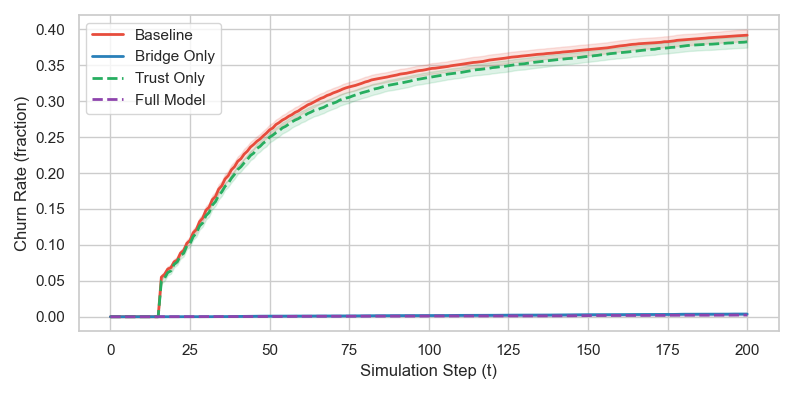
\includegraphics[width=0.58\textwidth]{figures/fig3_churn_factorial.png}
    \caption{Cumulative user churn rate over time ($N=500$, $30$ runs per condition). Filter Only mean final churn is $0.38\%$; Full Model is $0.21\%$; Filter OFF conditions show high attrition ($\approx 39\%$). Error ribbons: $95\%$ CIs.}
    \label{fig:churn}
\end{figure}

Mean frustration among active users falls to $0.5819$ ($\text{SD} = 0.0576$, $95\%\ \text{CI} = [0.5617, 0.6024]$, $W = 2.0$, $p_{\text{adjusted}} < 3.5 \times 10^{-7}$, $d = 3.08$). Step-wise revenue rises to \$199.24 ($\text{SD} = \$0.61$, $95\%\ \text{CI} = [\$199.03, \$199.45]$, $W = 0.0$, $p_{\text{adjusted}} < 1.1 \times 10^{-4}$). The $\approx \$78$ mean increase is demographic retention under fixed $M_{\text{unsafe}}=0.4$: because $\sigma(0)\approx 0.7 > \tau_{\text{cliff}}=0.6$, the stylized cliff does not switch in the main $2\times2$.

\subsubsection{Active-Agent Polarization and Full-Cohort Robustness}
Active-agent $\sigma$ rises from $0.9550$ ($\text{SD} = 0.0389$, $95\%\ \text{CI} = [0.9409, 0.9683]$) in Baseline to $0.9904$ ($\text{SD} = 0.0042$, $95\%\ \text{CI} = [0.9888, 0.9918]$) under Filter Only (mean difference $+0.0353$; $W = 12.0$, $p_{\text{adjusted}} < 8.1 \times 10^{-6}$, $|d| = 1.28$ with $d = -1.28$ under Group1$=$Baseline, Group2$=$Filter Only; Figure~\ref{fig:polarization}). Baseline exit removes extreme agents from the active set; the filter retains them.

\begin{figure}[htbp]
    \centering
    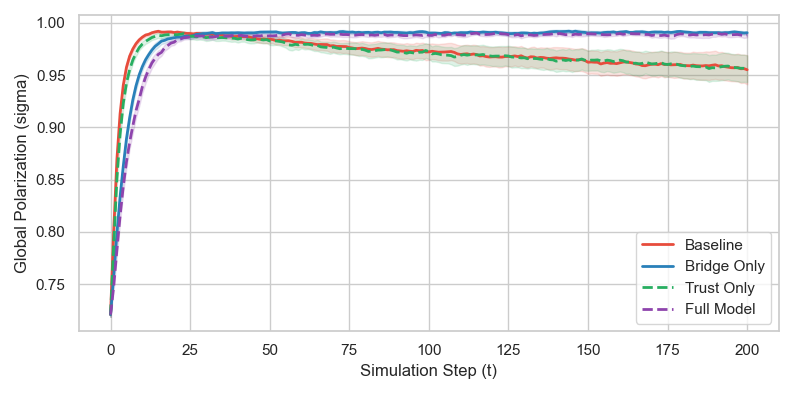
\includegraphics[width=0.58\textwidth]{figures/fig2_polarization_factorial.png}
    \caption{Active-agent polarization ($\sigma$) over time. Filter Only locks survivor polarization higher ($\sigma \approx 0.9904$) than Baseline ($\sigma \approx 0.9550$). This is an active-set / survivorship effect, not a full-population warming (see $\sigma_{\mathrm{all}}$). Error ribbons: $95\%$ CIs.}
    \label{fig:polarization}
\end{figure}

Full-cohort $\sigma_{\mathrm{all}}$ shows no Filter contrast: $0.9904$ vs.\ $0.9905$ ($W = 194.0$, $p_{\text{adjusted}} = 1.000$, $d = -0.004$). Retention effects remain; the claim that the filter \emph{raises} polarization applies to the active-user KPI matching the exit story.

\subsection{Trust Segregation}
Under \textbf{Trust Only}, ingroup trust rises to $0.9808$ ($\text{SD} = 0.0056$, $95\%\ \text{CI} = [0.9788, 0.9827]$) and outgroup trust falls to $0.0432$ ($\text{SD} = 0.0256$, $95\%\ \text{CI} = [0.0348, 0.0528]$; Figure~\ref{fig:trust_seg}). Trust Segregation averages $31.28$ ($\text{SD} = 18.83$, $95\%\ \text{CI} = [24.97, 38.21]$; median $= 26.76$, $\text{IQR} = [17.09, 40.66]$). Versus Baseline: $W = 0.0$, $p_{\text{adjusted}} < 1.2 \times 10^{-7}$ (complete same-direction separation; Baseline segregation is fixed at $1$ when Trust OFF). These contrasts enable trust co-evolution; they are not Filter effects.

\begin{figure}[htbp]
    \centering
    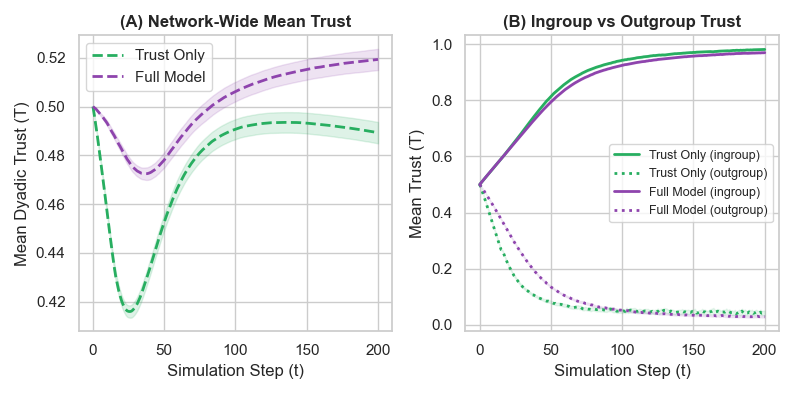
\includegraphics[width=0.65\textwidth]{figures/fig6_trust_dynamics.png}
    \caption{Dyadic trust dynamics. Panel A: mean trust under Trust Only and Full Model. Panel B: ingroup trust (near $0.98$) vs.\ outgroup trust (near $0.04$). Error ribbons: $95\%$ CIs.}
    \label{fig:trust_seg}
\end{figure}

\subsection{Moderation Analysis: Filter \texorpdfstring{$\times$}{x} Trust}
Seed-paired contrasts:
\begin{align}
    \Delta_{\text{alone}} &= \text{Metric}(\text{Filter Only}) - \text{Metric}(\text{Baseline}) \\
    \Delta_{\text{with trust}} &= \text{Metric}(\text{Full Model}) - \text{Metric}(\text{Trust Only})
\end{align}
Wilcoxon tests on $\Delta_{\text{with trust}}-\Delta_{\text{alone}}$ use a separate interaction Bonferroni family of size $m=7$ after excluding trust-KPI rows with $\Delta_{\mathrm{alone}}\equiv 0$ (Table~\ref{tab:interaction}). Those excluded rows are descriptive Full-vs-TrustOnly contrasts on trust metrics, not Filter$\times$Trust moderation. Same-pole triangle purity is included in the family (CSV column \texttt{Opinion\_Clustering}); its interaction is non-significant ($W=168$, adj.\ $p=1$).

\begin{table}[htbp]
\centering
\footnotesize
\caption{Filter $\times$ Trust interaction (seed-paired). Interaction family $m=7$ excludes trust-KPI rows with $\Delta_{\mathrm{alone}}=0$ (shown below the rule for transparency; adj.\ $p$ n/a). Active Users / Churn / Revenue are dependent retention readouts.}
\label{tab:interaction}
\begin{tabular}{lccccc}
\toprule
 & \textbf{Effect Alone} & \textbf{Effect w/Trust} & \textbf{Interaction} & & \\
\textbf{Metric} & \textbf{($\Delta_{\text{alone}}$)} & \textbf{($\Delta_{\text{with trust}}$)} & \textbf{Cohen's $d$} & \textbf{$W$} & \textbf{Adj.\ $p$} \\
\midrule
Active Users & $+194.0$ & $+190.3$ & $-0.3347$ & $117.5$ & $0.1250$ \\
Avg.\ Frustration & $-0.3849$ & $-0.3915$ & $-0.0368$ & $216.0$ & $1.0000$ \\
Churn Rate & $-38.80\%$ & $-38.05\%$ & $+0.3347$ & $121.0$ & $0.1523$ \\
Same-pole purity & $-0.0486$ & $-0.0446$ & $+0.2086$ & $168.0$ & $1.0000$ \\
Polarization ($\sigma$) & $+0.0353$ & $+0.0336$ & $-0.0469$ & $208.0$ & $1.0000$ \\
Polarization ($\sigma_{\mathrm{all}}$) & $+0.0000$ & $-0.0002$ & $-0.0382$ & $221.0$ & $1.0000$ \\
Revenue & $+\$77.60$ & $+\$76.11$ & $-0.3347$ & $111.0$ & $0.0871$ \\
\midrule
Ingroup Trust$^{\dagger}$ & $0.0000$ & $-0.0110$ & $-3.2083$ & $1.0$ & n/a \\
Mean Trust$^{\dagger}$ & $0.0000$ & $+0.0300$ & $+4.9482$ & $0.0$ & n/a \\
Outgroup Trust$^{\dagger}$ & $0.0000$ & $-0.0139$ & $-0.9249$ & $84.0$ & n/a \\
Trust Segregation$^{\dagger}$ & $0.0000$ & $+5.3710$ & $+0.4417$ & $135.0$ & n/a \\
\bottomrule
\multicolumn{6}{l}{\footnotesize $^{\dagger}$ Excluded from Bonferroni $m$: Trust OFF forces $\Delta_{\mathrm{alone}}=0$ (descriptive only).} \\
\end{tabular}%
\end{table}

Retention interactions (Active Users, Churn, Revenue---dependent readouts---and Frustration) remain non-significant after Bonferroni. Some raw $p$-values are $\approx 0.01$--$0.02$ before correction and then fail the $m=7$ family; with $n=30$ we report \emph{no evidence of moderation}, not statistical equivalence of Filter effects with and without trust. Active $\sigma$ likewise shows no Filter$\times$Trust interaction ($W=208$, adj.\ $p=1$).

\subsection{Echo Chambers}
Same-pole triangle purity (local closed active triples; Figure~\ref{fig:clustering}) averages $0.1316$ in Baseline ($\text{SD} = 0.0255$, $95\%\ \text{CI} = [0.1228, 0.1407]$); Trust Only $0.1316$ ($W = 226.0$, $p_{\text{adjusted}} = 1$). Filter Only lowers purity to $0.0830$ ($\text{SD} = 0.0152$, $95\%\ \text{CI} = [0.0776, 0.0884]$, $W = 0.0$, $p_{\text{adjusted}} < 1.2 \times 10^{-7}$, $|d| = 2.32$). Full Model: $0.0870$ ($\text{SD} = 0.0136$, $95\%\ \text{CI} = [0.0821, 0.0919]$, $W = 0.0$, $p_{\text{adjusted}} < 1.2 \times 10^{-7}$, $|d| = 2.19$). The filter can reduce local mono-pole triangles while active-agent $\sigma$ stays high---another active-set / KPI nuance.

\begin{figure}[htbp]
    \centering
    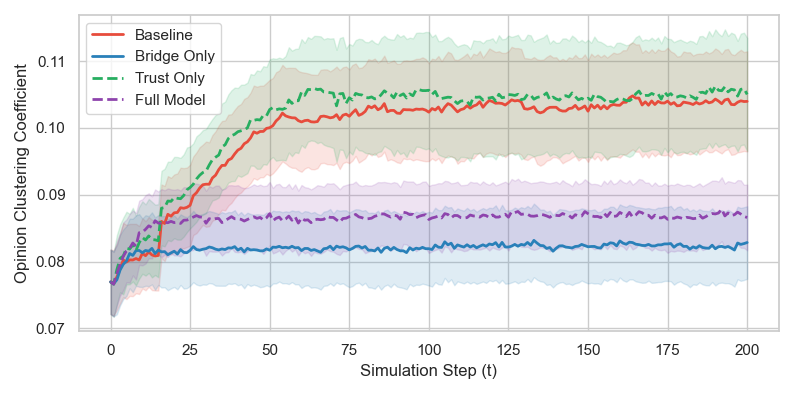
\includegraphics[width=0.58\textwidth]{figures/fig7_echo_chambers.png}
    \caption{Same-pole triangle purity (local closed active triples). Filter ON conditions reduce local mono-pole triangles relative to Baseline while active-agent polarization remains high. Error ribbons: $95\%$ CIs.}
    \label{fig:clustering}
\end{figure}

\subsection{Mechanism Checks}
Descriptive ablations ($20$ seeds; Figure~\ref{fig:ablations}; lower power than the main factorial). Relative to REF (churn $38.66\%$, $\sigma=0.9579$), intercept+heal (M0) yields churn $0.39\%$ and $\sigma=0.9901$. Heal-only (M1) yields churn $5.82\%$. Drop without heal (M2) and intercept with $B_{hb}=0$ (M3) are \emph{identical per seed} under current code (both churn $20.53\%$, $\sigma=0.9839$)---one mechanism identity, not two independent confirmations---and remain distinct from M0. Full Model without trust decay (M4) keeps near-zero churn. Setting the revenue multiplier to $1.0$ (M5) leaves polarization/churn unchanged but scales revenue to the full active-user level.

\begin{figure}[htbp]
    \centering
    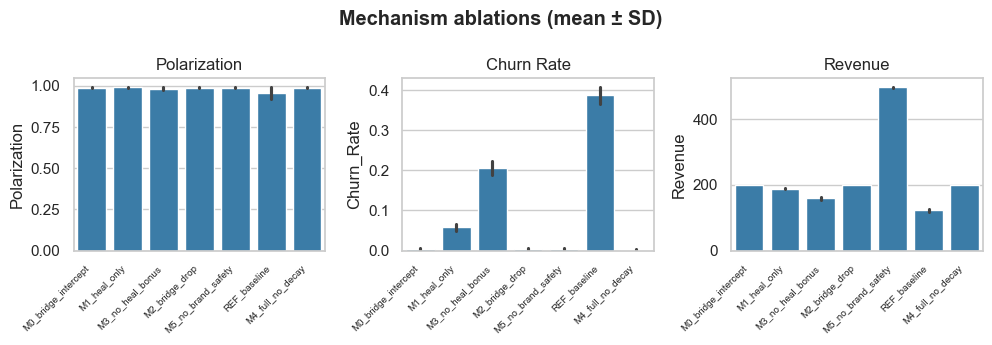
\includegraphics[width=0.95\textwidth]{figures/fig_ablations.png}
    \caption{Mechanism ablations ($20$ seeds): mean Polarization, Churn Rate, and Revenue. Error bars: SDs. Descriptive only.}
    \label{fig:ablations}
\end{figure}

\subsection{Baseline Model Comparison}
On the same BA networks and seeds, HK bounded confidence yields lower final polarization (mean $0.6991$) and no churn pathway. A lightweight biased-assimilation update without SJT zones or exit stays near-extreme (mean $0.9900$) with zero churn. Dynamic-BABE Baseline jointly produces high polarization and substantial exit (Figure~\ref{fig:baselines}).

\begin{figure}[htbp]
    \centering
    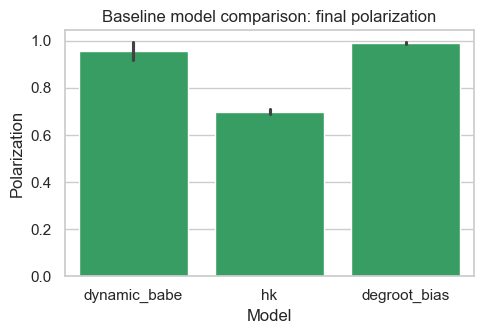
\includegraphics[width=0.55\textwidth]{figures/fig_baselines_polarization.png}
    \caption{Final polarization under Dynamic-BABE Baseline, Hegselmann--Krause, and biased DeGroot-style updates ($20$ seeds).}
    \label{fig:baselines}
\end{figure}

\subsection{Topology Robustness}
Filter OFF/ON on Watts--Strogatz ($k=6$, $p=0.1$; $15$ seeds; descriptive) preserves the qualitative direction: filter cuts churn while active-agent polarization rises, comparable to Barab\'{a}si--Albert under the same seeds (Figure~\ref{fig:topology}).

\begin{figure}[htbp]
    \centering
    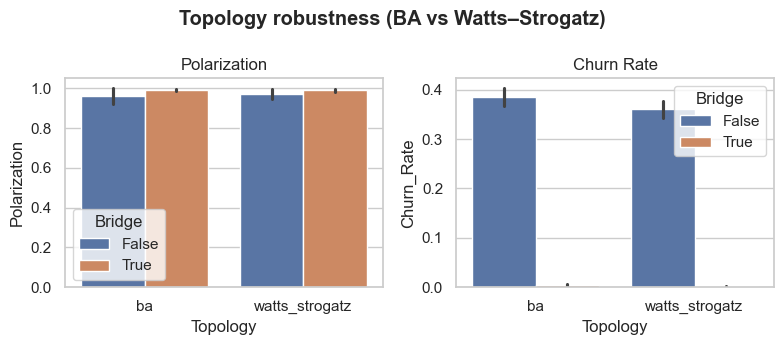
\includegraphics[width=0.85\textwidth]{figures/fig_topology_robustness.png}
    \caption{Filter OFF/ON contrasts on Barab\'{a}si--Albert vs.\ Watts--Strogatz ($15$ seeds). Descriptive.}
    \label{fig:topology}
\end{figure}


\section{Discussion}
\label{sec:discussion}
% paper/sections/07_discussion.tex
% Discussion Section

The quantitative results of our simulation experiments reveal a complex, co-evolutionary system where algorithmic content moderation, individual cognitive biases, and dyadic relational structures interact in unexpected ways. This section interprets these findings, linking our observations to established sociological and economic frameworks, examining the systemic trade-offs of dyadic trust, discussing the practical implications for social media architecture, and outlining the limitations that pave the way for future research.

\subsection{The Polarization Paradox: An Exit-Voice-Loyalty Analysis}
To understand the systemic mechanism of the Polarization Paradox, we analyze our findings through the lens of \citet{Hirschman1970} classic economic and political framework: \textit{Exit, Voice, and Loyalty}. Hirschman posits that when a system's quality declines (in this case, the rise of communicative toxicity on a social network), its members have two primary recovery paths: \textbf{Exit} (leaving the organization or platform permanently) or \textbf{Voice} (speaking up, debating, or actively working to resolve the conflict and restore quality).

In the Baseline condition of our model, the platform operates without any moderation filters. Entrenched agents are exposed to highly discrepant, cross-cutting views from their ideological outgroup. Lacking a protective trust buffer, these encounters fall into their Latitude of Rejection, triggering intense backfire cascades that drive opinions toward the extremes. Crucially, these backfires generate psychological friction, which accumulates as behavioral frustration. Because there is no mechanism to resolve these disagreements, agents eventually choose the path of \textbf{Exit}---they permanently churn. 

From the platform's perspective, this exit cascade is a disaster: it drains the active user base and collapses ad revenue. However, from a purely analytical standpoint, this mass exit acts as a natural pressure-valve for global polarization. The highly extreme, dogmatic agents exit the network, mathematically truncating the extremes of the opinion distribution and preventing the network from reaching absolute polarization.

When the platform deploys the bridging algorithm, it attempts to solve this economic threat. By probabilistically intercepting backfires and neutralizing their negative affect, the algorithm successfully blocks the \textbf{Exit} pathway. Users are spared the frustration of toxic conflict, and they remain active, generating continuous advertising revenue. 

Crucially, however, the bridging algorithm does not promote \textbf{Voice}. The algorithm does not help users resolve their disagreements; rather, it replaces a hostile backfire with silence (Zone 2, non-commitment). By neutralizing cross-cutting dialogue, the platform effectively forces its users into a state of passive \textbf{Loyalty}---they remain on the platform and generate profit, but they are relationally and ideologically frozen. 

This leads to the paradox: because the exit valve is closed and the voice valve is blocked, the highly extreme and entrenched agents remain active in the network indefinitely. These extreme users continue to pull their locally connected neighbors toward the ideological poles, locking the system into an absolute, structural polarization. The platform successfully monetizes this passive loyalty, but at the cost of relationally hollowing out the social network and entrenching systemic polarization.

\subsection{The Double-Edged Sword of Dyadic Trust}
Our introduction of a dynamic, co-evolving dyadic trust system reveals that trust is a double-edged sword in social networks. On one hand, trust acts as a powerful constructive glue within ideological camps. The co-evolutionary mechanism allows like-minded agents to build deep relational capital ($\delta_+ = 0.02$). This high ingroup trust ($0.9814$) acts as a strong cognitive buffer, shifting the influence weight $w_{ij}$ upward. This buffer allows agents to engage in constructive dialogue even when they disagree on specific issues, facilitating consensus and smoothing over minor internal ideological differences.

On the other hand, the asymmetry of trust co-evolution ($\delta_- / \delta_+ = 2.5$) acts as a highly destructive solvent across ideological camps. Because trust is fragile---easy to lose and exceptionally difficult to rebuild \citep{Slovic1993}---confrontational cross-camp interactions rapidly eradicate outgroup trust ($0.0415$). 

Combined with passive decay ($\lambda = 0.001$), this rapid erosion leads to a severe relational balkanization, where the network is partitioned into two mutually hostile silos with an average Trust Segregation Ratio of $35.61$. In this segregated landscape, outgroup agents have no relational capital, meaning their opinions are completely discounted, further entrenching the global ideological division.

\subsection{Platform Design and Architectural Implications}
These findings have profound implications for the design of modern social media architectures. Current algorithmic moderation systems primarily optimize for short-term engagement, user retention, and brand safety. When platforms deploy bridging algorithms or content suppression filters, they are essentially treating the behavioral symptoms of polarization (toxic conflict and user exit) rather than its underlying cognitive and relational causes (deep ideological entrenchment and fragile trust).

Our model demonstrates that this symptom-based intervention leads to a highly fragile, relationally hollowed-out network. By hiding conflict and promoting mutual isolation, platforms create a silent, highly segregated echo chamber. While this strategy successfully protects ad rates and keeps active user counts high, it systematically destroys the relational capital necessary for cross-ideological understanding.

To move beyond the Polarization Paradox, platform designers must adopt **multi-objective algorithmic optimization**. Algorithms should optimize not just for short-term active sessions or the absence of conflict, but for long-term relational capital and cross-camp trust. 

Rather than suppressing cross-cutting views, platforms should deploy algorithms that actively facilitate constructive, trust-building contact. For example, instead of matching agents based on raw ideological similarity, algorithms could pair users based on shared salience weights on non-controversial issues (e.g., matching a progressive and a conservative who both care deeply about local sports or community volunteerism). 

By building initial trust on shared dimensions, the platform can establish the relational buffer necessary to withstand subsequent political disagreements, transforming toxic outgroup hostility into constructive democratic voice.

\subsection{Limitations and Future Work}
While the Dynamic-BABE model offers critical theoretical insights into social networks, it possesses several simplify constraints that present opportunities for future research:
\begin{enumerate}
    \item \textbf{Symmetric Trust:} Our current formulation assumes that dyadic trust is strictly symmetric ($T_{ij} = T_{ji}$). In real-world relationships, trust is often asymmetric: one individual may trust a public figure or a friend far more than they are trusted in return. Future work should relax this constraint to explore how asymmetric trust vectors and directed relational networks impact opinion convergence.
    \textbf{Static Network Topology:} The Barab\'{a}si-Albert network topology remains static throughout our simulations. In actual social media environments, agents dynamically alter their communication structures through homophilous rewiring (e.g., unfriending, blocking, or following others based on ideological compatibility). Integrating dynamic network rewiring would allow researchers to study the co-evolution of opinions, trust, and physical topology.
    \item \textbf{Low-Dimensional Issue Space:} We model opinion dynamics across $K=2$ dimensions. While this captures the primary axis of social discourse, real-world political landscapes are high-dimensional, involving multiple overlapping, shifting issues. Future models should scale the issue dimensions to investigate how multidimensional consensus and cross-cutting cleavages affect global polarization.
    \item \textbf{Empirical Calibration:} The agent cognitive and behavioral parameters (such as $\beta_i$, $\tau_{\text{assim}}$, and $\delta_-$) are grounded in social judgment and cognitive literature, but they are not calibrated to specific empirical platform datasets. Future work should use empirical data from platforms like Twitter/X or Reddit to calibrate cognitive parameters and validate the emergent polarization trends.
\end{enumerate}
Despite these limitations, the Dynamic-BABE model provides a powerful, mathematically rigorous foundation to understand how algorithmic systems and cognitive processes interact to shape the relational fabric of modern society.


\section{Conclusion}
\label{sec:conclusion}
% paper/sections/08_conclusion.tex

Dynamic-BABE links opinion dynamics, dyadic trust, exit, and a stylized Suppression Filter. Under our defaults, the filter sharply improves retention and retention-scaled revenue while raising \emph{active-agent} polarization by keeping extreme agents who would otherwise exit; full-cohort $\sigma_{\mathrm{all}}$ does not show that rise. Trust co-evolution separately produces trust segregation. Seed-paired Filter $\times$ Trust analyses suggest retention benefits are robust to trust, whereas relational moderation should be read cautiously---especially for trust KPIs that are undefined when Trust OFF.

The practical implication is modest: retention and cohesion among remaining users need not move together when disagreement is suppressed and trust is fragile. Designs that only minimise visible conflict may miss relational outcomes that matter for long-run tolerance. Escaping the paradox, if that is the goal, requires contact conditions under which trust can form---not only filters that prevent rejection-zone events.


\section*{Code and Data Availability}
An anonymised replication archive (model code, batch scripts, analysis pipeline, and figure generators) will be provided to the editors for peer review. Upon acceptance, a reviewed release will be deposited on the CoMSES Net Computational Model Library so that a permanent handle can accompany the published article.

\endparano

\theendnotes

\bibliographystyle{jasssbib}
\bibliography{references}

\end{document}
